\documentclass{article} % kind of document 
\usepackage[utf8]{inputenc} %encoding of choice
\usepackage[american]{babel} %language of choice
\usepackage[p,osf]{cochineal}
\usepackage{fancyhdr} %for header
\usepackage{amsmath, tabu} %math mode
\usepackage{mathtools}
\usepackage{amssymb} %math symbols
\usepackage{dsfont} %specifically for the indicator function symbol
\usepackage{xcolor} %to color text
\usepackage{amsthm} %math theorem
\usepackage{tikz}
\usepackage{caption}
\usepackage{multirow}
\usepackage[bottom]{footmisc}
% \usepackage[dvipsnames]{xcolor}
\usepackage{enumerate} %make lists
\usepackage{graphicx} %insert images
\usepackage{float} %to fix image position
\usepackage{moreverb} %to make boxes
\usepackage{hyperref} %to create hyperlinks
\usepackage{lipsum} %lorem ipsum package
\usepackage{setspace} % to use singlespace below in the solution environment
\usepackage[shortlabels]{enumitem}
\usepackage{parskip}
\usepackage[us]{datetime} %package for setting due date in US format
\newdate{duedate}{15}{09}{2021} %to set a due date
\allowdisplaybreaks
\usepackage[margin=1in]{geometry}
\pagestyle{fancy}


\lhead{Due: \displaydate{duedate}}
\chead{ECON 899 -- Problem Set 1}
\rhead{Yobin}

%\DeclareUnicodeCharacter{00A0}{ }


\DeclareMathOperator*{\E}{\mathbb{E}} %ease of writing e and E
\newcommand{\e}{\mathrm{e}}
\newcommand{\ct}{\mathsf{c}}
\newcommand{\Z}{\mathbb{Z}}
\newcommand{\R}{\mathbb{R}}
\newcommand{\N}{\mathbb{N}}
\newcommand{\ifn}{\mathds{1}}
\newcommand{\X}{\mathbf{X}}
\newcommand{\Y}{\mathbf{Y}}
\newcommand{\one}{\mathbf{1}}
\newcommand\numberthis{\addtocounter{equation}{1}\tag{\theequation}}
\newcommand*\widebar[1]{\overline{#1}} % to get a widebar
\theoremstyle{definition}
\newtheorem{theorem}{theorem} % Theorem display format
\newtheorem{problem}[theorem]{Exercise} % Problem display format, last bracket sets display choice

\newenvironment{solution}[1][Answer]{\begin{singlespace}\underline{\textbf{#1:}}\quad }{\ \rule{0.3em}{0.3em}\end{singlespace}} % Answer format

\newenvironment{solutions}[1][Proof]{\begin{singlespace}\underline{\textbf{#1:}}\quad }{\ \rule{0.3em}{0.3em}\end{singlespace}} % Answer format

\begin{document}
	Assume that households have log preferences, the production technology satisfies $Y_t = Z_tK_t^\alpha$ where $\alpha = 0.36$; and capital depreciates at rate $\delta = 0.025$. We will
	assume technology shocks follow a 2 state Markov Process. The transition matrix is calibrated to NBER business cycle data where we take an expansion to be an instance of a positive technology shock and recession to be an instance of a negative technology shock. The transition matrix is given by
	\[\begin{bmatrix}
		0.977 & 0.023 \\0.074 & 0.926
	\end{bmatrix}\]

\underline{Comment on computation time:} \textit{The stochastic code on Julia converged after 434 iterations and took 4.95 seconds to run.}

\begin{enumerate}
	\item State the dynamic programming problem.
	\begin{solution}
		The dynamic programming problem can be stated as:
		\begin{align*}
			V(K,Z) = \max_{C,K'} \{ \log(C) + \beta \E[V(K',Z')|Z] \} \;\; \text{s.t. } \;\; C + K' = ZK^\alpha + (1 - \delta)K
			\intertext{which can be rewritten as an dynamic optimization problem of one variable as}
			V(K,Z) = \max_{K'} \{ \log(ZK^\alpha + (1 - \delta)K - K') + \beta \E[V(K',Z')|Z] \}
		\end{align*}
	\end{solution}
	\item Plot the value function $K$ over each state $Z$. Is it increasing (i.e. is $ V(K_{i+1}, Z) \geq V(K_i,Z) $) for $ K_{i+1}  > K_i $? Is it concave?
	\begin{solution}
		
		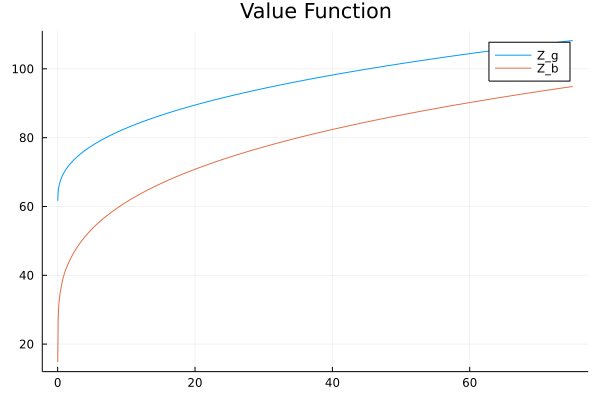
\includegraphics[width=\linewidth]{02_Value_Functions.png}
		
		The value function appears to be strictly increasing and concave.
	\end{solution}
	
	\item Is the decision rule increasing in $ K $ and $ Z $ (i.e. is $K'(K_{i+1}, Z) \geq K'(K_i, Z)$ for $ K_{i+1} > K_i $  and is $ K'(K,Z^g) \geq K'(K,Z^b)$)? Is savings increasing in $ K $ and $ Z $ (to see this, plot the change in the decision rule $ K'(K,Z) - K $ across $ K $ for each possible exogenous state Z)?
	\begin{solution}
		The decision rule is indeed increasing in $ K $ and $ Z $ (since the $ Z_g $ line is higher than the $ Z_b $ line for all values of $ K $).
		
		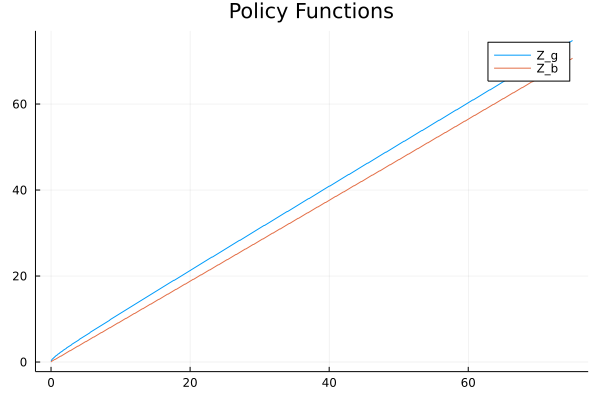
\includegraphics[width=\linewidth]{02_Policy_Functions.png}
		
		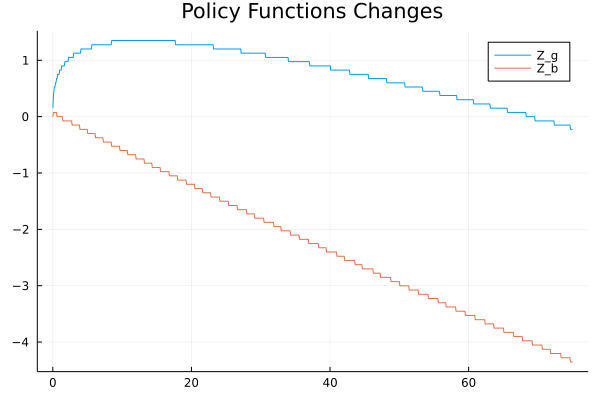
\includegraphics[width=\linewidth]{02_Policy_Functions_Changes.png}
		
		Savings is indeed increasing in $ Z $. It is decreasing in $ K $ for $ Z_b $. And it is increasing for lower levels of $ K $ over $ Z_g $   but decreasing for higher levels of $ K $. That is, even with the realization of a good technology shock, savings decision depends on agent's values of $ K $. Agents with large capital stock want to dissave whereas those with low stock want to save.
	\end{solution}
\end{enumerate}
\end{document}